\chapter{Extrañeza}\label{cap:strangeness}
Como se comentó anteriormente, los físicos británicos George Rochester y Clifford Butler se hallaban tomando fotografías en una cámara de niebla en 1947, tratando de detectar partículas generadas por los rayos cósmicos al impactar sobre las moléculas de la atmósfera, cuando detectaron dos rastros en forma de $V$ invertida nunca observados hasta entonces, que sólo podían ser explicados por el decaimiento de una partícula neutra con masa entre 700 y 1600 veces mayor a la del electrón. 

En aquella época, ante la ausencia de aceleradores de partículas potentes, la búsqueda de partículas se realizaba estudiando los rayos cósmicos. Estos rayos no son más que radiación de alta energía procedente del espacio exterior. Cuando estos inciden en las distintas capas de la atmósfera producen una serie de reacciones en cadena que da lugar a una cascada de partículas. Además, a mayor altitud, mayor es el flujo de rayos cósmicos que nos llegan, lo que facilita que un mayor número de partículas llegue al detector. Por este motivo, Rochester y Butler decidieron realizar nuevamente el experimento en los Pirineos Franceses, concretamente en el observatorio \textit{Pic Du Midi}, y esta vez consiguieron detectar decenas de estas nuevas partículas. En un principio se las denominó partículas $V$ pero posteriormente pasaron a identificarse como mesones $\PK$ o kaones \cite{Griffiths2008}.

Para entender cómo lograron detectar los mesones $\PK$ por primera vez, hay que entender el funcionamiento de las cámaras de niebla. Estos dispositivos son entornos cerrados donde se llevaba a cabo el estudio de los rayos cósmicos: las partículas que componen los rayos atraviesan un volumen con vapor de agua sobresaturado contenido en dicho recinto cerrado. Las partículas con carga eléctrica producen una cierta ionización de aire provocando la condensación del vapor de agua a lo largo de la trayectoria.  Al situar la cámara de niebla en campos electromagnéticos y, estudiando las curvaturas de las trayectorias, es posible obtener la carga eléctrica, la energía y la masa de las partículas.  Asimismo, como muchas partículas decaen en otras por ser inestables, estudiando la longitud de las trazas que dejan tras decaer en la cámara de niebla, pueden deducirse sus vidas medias \cite{notas2020}.

En diciembre de 1947, se publicaron en la revista \textit{Nature} dos de las numerosas fotografías tomadas por Rochester y Butler, que se observan a continuación:

\begin{figure}[h!]
	\centering
	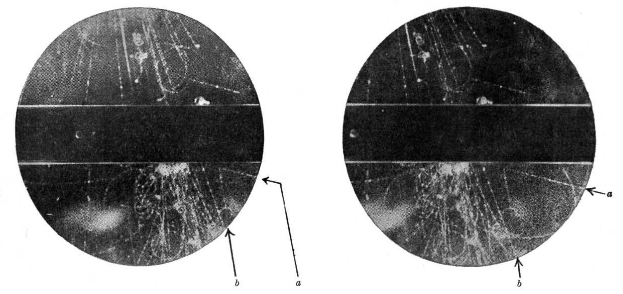
\includegraphics[width=0.8\textwidth]{C:/Users/Carmen/Desktop/Universidad/TFG/Borradores/img/rochester1.PNG}
	\caption[Fotografía 1 de la primera detección de los mesones $\PK$]
	{Primera fotografía estereoscópica publicada en la revista \textit{Nature} \cite{Nature1},}
	\label{fig:nature1}
\end{figure}
\begin{figure}[h!]
	\centering
	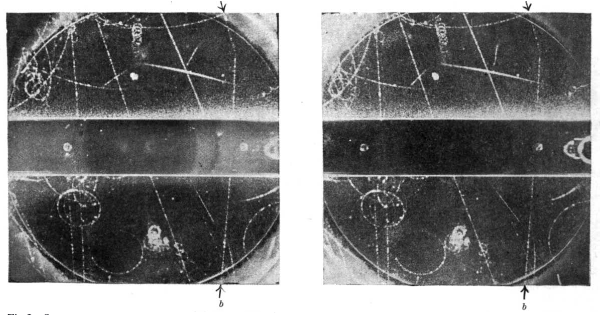
\includegraphics[width=0.7\textwidth]{C:/Users/Carmen/Desktop/Universidad/TFG/Borradores/img/rochester2.PNG}
	\caption[Fotografía 2 de la primera detección de los mesones $\PK$]
	{Segunda fotografía estereoscópica publicada en la revista \textit{Nature} \cite{Nature1}.}
	\label{fig:nature2}
\end{figure}

En la figura \ref{fig:nature1}, se observa como las partículas de rayos cósmicos entran por la parte superior izquierda y colisionan contra la placa de plomo, produciendo una partícula neutra, cuya presencia se hace evidente al decaer en otras partículas cargadas más ligeras, formando una ``V'' invertida en la parte inferior derecha, señalada mediante las marcas a y b. La figura \ref{fig:nature2} muestra un proceso similar pero esa vez, se produce una nueva partícula cargada que decae en otras dos partículas más ligeras, una cargada y otra neutra, apreciándose una V más abierta, como una desviación en la trayectoria.

Para entender las fotografías en mayor detalle, la figura \ref{fig:esquema1} muestra un esquema de ambos procesos.

\begin{figure}[h!]
	\centering
	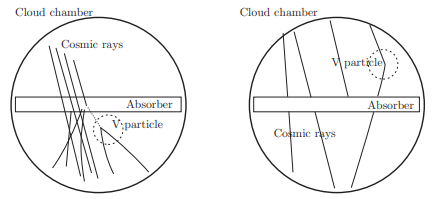
\includegraphics[width=0.65\textwidth]{C:/Users/Carmen/Desktop/Universidad/TFG/Borradores/img/esquema.PNG}
	\caption[Esquema para entender las fotos estereoscópicas]
	{Esquema de los procesos observados en las fotografías anteriores \cite{Franzini}.}
	\label{fig:esquema1}
\end{figure}

Años más tarde se comprobó que la primera fotografía \ref{fig:nature1} correspondía al proceso  $\PKz \rightarrow \Pgpp$ +  $\Pgpm$ y la segunda fotografía (\ref{fig:nature2}) a la reacción $\PKp \rightarrow \APmuon$ + $\Pnu$.

El comienzo de los años 50 trajo consigo técnicas innovadoras de detección de partículas, como la cámara de burbujas, detectores de emulsión nuclear muy precisos y nuevos aceleradores más potentes. Estos nuevos dispositivos demostraron un gran avance tecnológico al permitir la producción casi en masa de las partículas descubiertas en la década anterior. 

De hecho, los mesones $\PK$ habían quedado un poco en el olvido durante los dos años posteriores a su descubrimiento hasta que en 1950, otros célebres físicos de partículas como Powell, empezaron a publicar trabajos donde también se apreciaban los trazos en forma de $V$ y las desviaciones, que evidenciaban la presencia de las partículas $V$. Coincidían con Rochester y Butler en que estos eventos representaban el decaimiento espontáneo de partículas neutras y cargadas, desconocidas hasta entonces \cite{Pais}. 

\begin{figure}[h!]
	\centering
	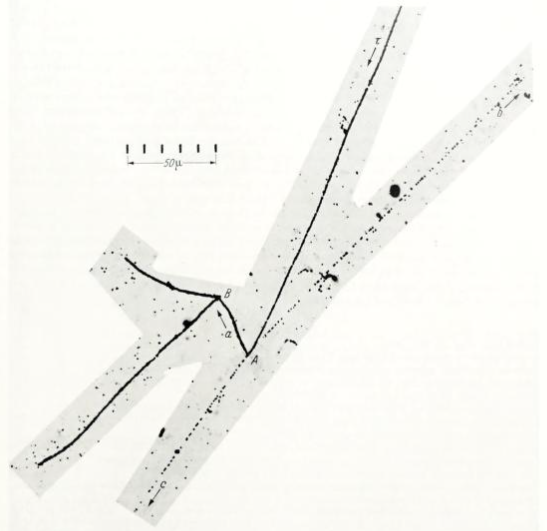
\includegraphics[width=0.5\textwidth]{C:/Users/Carmen/Desktop/Universidad/TFG/Borradores/img/powell2.PNG}
	\caption[Fotografía de Powell mostrando una desviación en la trayectoria]
	{Fotografía publicada por el grupo de Powell \cite{Griffiths2008}.}
	\label{fig:powell}
\end{figure}

El proceso descubierto por Powell en \ref{fig:powell} mostraba como $\PKp$ entrando desde arriba decae en el punto A en tres piones cargados, dos positivos y uno negativo. El $\Pgpm$ provoca seguidamente una desintegración en B. El proceso descrito era: $\PKp \rightarrow \Pgpp$ + $\Pgpp$ +  $\Pgpm$.

Sin embargo, la partícula $\PKz$ de \ref{fig:nature1} primero fue conocida como $V^0$ y luego como $\theta^0$ antes de renombrarse finalmente como $\PKz$, mientras que la partícula $\PKp$ de \ref{fig:powell} se denominó en un principio como $\APtauon$. Esto es debido a que los procesos tenían estados finales con distinta paridad y, por dicha razón, se pensaba que debía tratarse de partículas diferentes.

Las partículas $\theta^0$ y $\APtauon$ no se identificaron como distintas versiones de una misma partícula hasta 1956, cuando se resolvió el conocido enigma $\tau$-$\theta$ al descubrir la violación de la paridad en la interacción débil \cite{Lee}, de la cual hablaremos más adelante. 

En los años siguientes se empezaron a clasificar las partículas $V$ y $\Ptau$ en función de la masa. Así, se determinó que los mesones $\PK$ correspondían a aquellas partículas con masa intermedia entre el pión y el protón, mientras que aquellas con masas intermedias entre el neutrón y el deuterón pasarían a conocerse como hiperones. 

Volviendo al inicio de los años 50, fue también entonces cuando empezaron a hacerse notar los fenómenos inusuales que presentaban estas partículas y que fueron los responsables de que se las bautizara como partículas extrañas, pues nunca se habían manifestado en otras partículas. Las partículas extrañas incluyen no sólo los mesones $\PK$, sino también los hiperones $\PLambda$, $\PSigma$ y cascada $\PXi$, entre otros. No obstante, en este trabajo vamos a centrar nuestro estudio en los kaones.

La primera característica extraña de estas partículas es que, a pesar de producirse por interacción fuerte de forma muy numerosa, tienen vidas medias relativamente largas, por lo que se sospechaba que decaían mediante interacción débil. La fuerza débil tiene un alcance muy corto (ver capítulo \ref{cap:weak_int}), por lo que requiere un tiempo más largo que otras interacciones para provocar la desintegración de la partícula. Básicamente, la vida media de una partícula es una indicación aproximada de cuanto tiempo necesita actuar la fuerza para producir el decaimiento. El otro suceso curioso es el de producción asociada, que consiste en que las partículas extrañas sólo se producen por pares.  

Tras muchos intentos fallidos de dar explicación a estos hechos, el físico holandés-estadounidense Abraham Pais sugirió, en 1952, que las partículas elementales debían tener una nueva propiedad o regla de selección, a la que denominó ``regla par-impar''. Esta regla de selección debía de cumplirse siempre para la interacción fuerte y la electromagnética, pero podía violarse en la interacción débil. A grandes rasgos, la regla consistía en asignar el número 0 a las partículas ``antiguas'' ($\Pgp$, nucleones, $\Pgg$, leptones) y el número 1 a las partículas ``nuevas'' $\PK$ y $\PLambda$ (el resto de las partículas todavía se desconocían). Dado cualquier proceso, se suman los números asignados de las partículas en el estado inicial y luego las del estado final. En la interacción fuerte y electromagnética, el número total inicial y final deben ser ambos pares o ambos impares, mientras que, en la interacción débil, uno debe ser par y el otro impar. Esta propiedad también daba respuesta a por qué las partículas extrañas debían producirse en pares \cite{Pais}.

La evidencia experimental de la idea de Pais vino de la mano de Murray Gell-Mann y Kazuhiko Nishijima en 1953. Por un lado, indicaban que la ``Regla par-impar'' debía ser una consecuencia directa de la independencia de carga de las partículas $V$, que indicaba que la carga de estas partículas podía encontrarse en tres estados: neutro, positivo y negativo. Por otro lado, Gell-Mann propuso asignar un número entero de isospín $I$ a los hiperones y un semientero a los mesones $\PK$. Nakano y Nishijima también hicieron esta misma propuesta casi paralelamente. Dependiendo de si $I$ y su tercera componente $I_3$ se conservan o no, podrán producirse partículas mediante interacción fuerte \cite{nakano}.

En 1955, Nishijima planteó, a partir de sus observaciones experimentales, que los mesones $\PK$ se podían organizar en dobletes de carga y, por tanto, podían obtenerse partículas $\PK$ con carga conjugada. $\PKp$ y $\PKz$ formaban un doblete de carga con $I=1/2$ e $I_3=1/2$ y $-1/2$ respectivamente y, además, ambas partículas podían definirse como funciones de onda complejas. Ello permitía establecer el doblete conjugado de sus antipartículas $\PKm$ y $\PaKz$, con $I_3=-1/2$ y $1/2$ respectivamente, relacionados entre sí mediante el operador conjugación de carga. Gell-Mann también llegó a conclusiones similares en 1956. Profundizaremos en mayor medida sobre este tema en los próximos capítulos \cite{Nishijima1955}.

Adicionalmente, se comprobó que en todas las interacciones antes descritas se conservaba el número bariónico $B$.\protect\footnotemark Asimismo, desarrollando toda esta teoría de la invariancia de carga para las partículas $V$ y para incluir la propiedad sugerida por Pais, se introdujo un nuevo número cuántico al que Gell-Mann denominó \textit{extrañeza} $S$ (Nishijima la denotó como carga-$\eta$).

\footnotetext{Las teorías de Unificación afirman que el protón $p$ tiene vida finita aunque muy larga. Si decae, lo haría en un $e^+$ y en un $\Pgpz$, violándose la conservación de $B$.}

Se asignó $S=1$ al doblete de partículas de mesones $\PK$ y $S=-1$ para el doblete de sus antipartículas. Este nuevo número cuántico resultaba últil para relacionar la carga con $I_3$ en partículas elementales, llegándose a una expresión conocida como la \textit{Fórmula de Gell-Mann-Nishijima}:

\begin{equation}
Q=I_3+ \frac{B+S}{2}=I_3+\frac{Y}{2} ,
\end{equation}
siendo $Y$ la \textit{hipercarga}, definida como $Y=B+S$.

La propiedad de conservación de la extrañeza se formuló a partir de las evidencias experimentales: $S$ debía conservarse en las interacciones fuerte y electromagnética, pero podía ser violada en procesos ocurridos por interacción débil, tal y como había sugerido Pais con su \textit{regla par-impar}.\\


\section{Extrañeza en el Modelo de Quarks}\label{cap:strangeness_quark_model}
%\vspace{3mm}
Como hemos visto, el concepto de extrañeza se introdujo por motivos puramente fenomenológicos, gracias a las observaciones experimentales. Sin embargo, a través del Modelo de Quarks, la extrañeza obtiene su base teórica.

A principios de la década de los 60 y tras el descubrimiento de muchas partículas ``elementales'', fue necesario poner cierto orden haciendo uso de las simetrías. Las simetrías son útiles porque permiten clasificar de forma ordenada las partículas en función de sus propiedades. La rama de las matemáticas encargada de tratar con simetrías es la teoría de grupos. El isospín viene descrito por el grupo $SU(2)$, pero el descubrimiento de las partículas extrañas hizo necesario extender el concepto de isospín a una simetría superior.

Así pues, Gell-Mann y Ne'eman observaron que los valores de isospín y la hipercarga de los hadrones estaban relacionados entre sí, tal que los hadrones (mesones y bariones) aparecían en grupos con el mismo espín y paridad y masas similares, denominados singletes (una partícula), octetes (ocho partículas) y decupletes (diez partículas).  Esta clasificación, que recibió el nombre de \textit{The Eightfold Way} o \textit{El Camino Óctuple}, concordaba con la estructura del grupo de simetría interna $SU(3)$ si fundamentaban las transformaciones en la independencia de carga de la interacción fuerte (isospín) y en la conservación de la extrañeza \cite{notas2020}. Las diversas representaciones del grupo $SU(3)$, no sólo permitían la clasificación de las partículas en función de sus números cuánticos, sino que además, predecían la existencia de nuevas partículas aún por descubrir. 

Pero entonces, ¿existía alguna razón profunda que proporcionase una explicación a la ordenación de las partículas de este modo? La respuesta a esta pregunta se obtuvo en 1964, cuando Gell-Mann y Zweig, plantearon la posibilidad de que estas partículas, que en un principio se creían elementales, podrían presentar una estructura interna más compleja, pues habían observado ciertas propiedades en ellas que así lo sugerían. Gell-Mann bautizó a estos entes más fundamentales que constituían las partículas como \textit{quarks} \cite{Griffiths2008}. El quark presentaba tres estados internos o ``sabores'', llamados $\Pup$ (\textit{up}), $\Pdown$ (\textit{down}) y $\Pstrange$ (\textit{strange}), cada uno con un determinado valor de carga y extrañeza. Además, indicó que para cada quark $\Pquark$, existía su correspondiente antiquark $\APquark$ con números cuánticos aditivos opuestos. En la siguiente tabla se puede observar un resumen de sus propiedades:

\begin{table}[h!]
	\centering
	\begin{tabular}{l*{8}{c}r}
\hline
Quark $(\Pquark)$ & Espín $s$ & Carga $Q$ & $I$ & $I_3$ & $S$ & $B$ & $Y$\\ 
\hline
Up $(\Pup)$ & $1/2$ & $+2/3$ & $1/2$ & $+1/2$ & $0$ & $1/3$ & $1/3$\\
Down $(\Pdown)$ & $1/2$ & $-1/3$ & $1/2$ & $-1/2$ & $0$ & $1/3$ & $1/3$\\
Strange $(\Pstrange)$ & $1/2$ & $-1/3$ & $0$ & $0$ & $-1$ & $1/3$ & $-2/3$\\
\hline
	\end{tabular}
\caption[Números cuánticos de los quarks]{Números cuánticos de los quarks \cite{notas2020}.} %\protect\footnotemark}
\label{tab:propiedades_quarks}
\end{table}

%\footnotetext{Recordemos que los respectivos antiquarks tienen números cuánticos opuestos.}

El \textit{Modelo de Quarks} describe la estructura de los bariones (antibariones) constituidos por un conjunto de tres quarks (antiquarks) mientras que los mesones están formados por un quark y un antiquark. El ``\textit{The Eightfold Way}'' sólo era una consecuencia de las simetrías de sabor de los quarks, matemáticamente expresada mediante la simetría del grupo $SU(3)$. Las diferentes combinaciones de sabor daban lugar a las distintas partículas y sus propiedades.

En concreto, los mesones $\PK$ se representaban junto a los piones en un hexágono que los clasifica según sus números cuánticos de carga $Q$ y extrañeza $S$, formando un octete pseudo-escalar.\footnote{Pseudo-escalar indica que los mesones tienen momento angular 0 y paridad negativa ($J^\pi = 0^-$).} Dicho octete está formado por el triplete de los piones y los dos dupletes de las partículas $\PK$ y sus antipartículas, aunando así todos los mesones ligeros en un mismo grupo. Para formar el octete de mesones, en cada vértice del hexágono se sitúa una partícula y en el centro del mismo se sitúan el pión neutro y el mesón $\Pgh$. La representación de este octete se muestra en la figura \ref{fig:octete}.

\begin{figure}[h!]
	\centering
	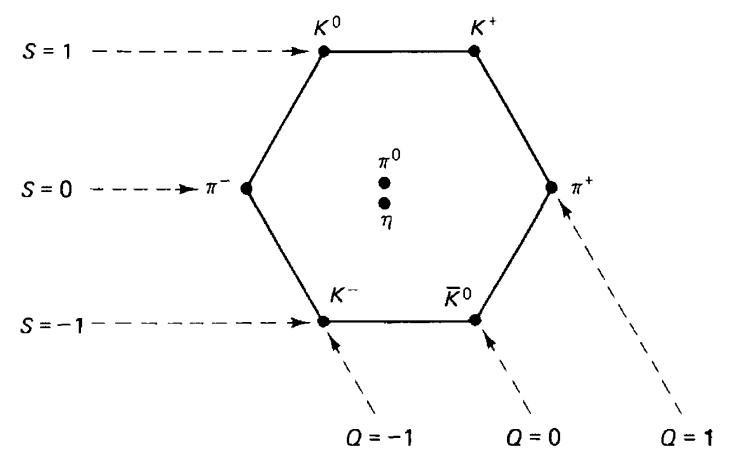
\includegraphics[width=0.65\textwidth]{C:/Users/Carmen/Desktop/Universidad/TFG/Borradores/img/octete.PNG}
	\caption[Octete de mesones]
	{Octete de mesones \cite{Griffiths2008}.}
	\label{fig:octete}
\end{figure}

El octete mesónico muchas veces aparece representado como un nonete para incluir las nueve posibles combinaciones de $\Pquark$ y $\APquark$, al incluir el singlete de la partícula $\Pghpr$.

Por lo tanto, todas aquellas partículas en cuya composición estuviera presente el quark $\Pqs$, como en los kaones, presentaban un valor de extrañeza no nulo y podían considerarse partículas extrañas. 

La composición de quarks de los mesones $\PK$ es la siguiente:

\begin{table}[h!]
	\centering
	\begin{tabular}{l*{2}{c}r}
\hline
Mesón & Quarks\\ 
\hline
$\PKp$ & $\Pqu\Paqs$\\
$\PKm$ & $\Pqs\Paqu$\\
$\PKz$ & $\Pqd\Paqs$\\
$\PaKz$ & $\Pqs\Paqd$\\
\hline
	\end{tabular}
\caption[Composición de quarks de los mesones $\PK$]{Composición de quarks de los mesones $\PK$ \cite{notas2020}.} 
\label{tab:mesonesK_quarks}
\end{table}

Conociendo esta composición y los números cuánticos de los quarks de la tabla \ref{tab:propiedades_quarks}, se obtienen fácilmente las propiedades de los mesones $\PK$ mostradas en la tabla \ref{tab:propiedades}.

Lo más destacable de los quarks es que son partículas fermiónicas, es decir, tienen espín $1/2$. Sin embargo, la existencia de los bariones requiere la agrupación de tres quarks y esto, en ciertas situaciones era incompatible con el \textit{Principio de Exclusión de Pauli}. Para resolver esta paradoja, Greenberg introdujo el concepto de color: además de los tres sabores de quarks, estos también presentan tres colores $r$ (\textit{red}), $b$ (\textit{blue}) y $g$ (\textit{green}). Planteó que los bariones simplemente se forman con quarks de distinto color. Por lo tanto, ya no serían exactamente iguales y no se violaría el Principio de Pauli \cite{Griffiths2008}. Además, aunque los quarks son los constituyentes más fundamentales de la materia, no se han encontrado evidencias de la existencia de quarks aislados, es lo que se conoce como confinamiento \cite{Pais}.

Con los años se han descubierto otros sabores de quarks, los llamados quarks pesados $\Pqc$ (\textit{charm}), $\Pqt$ (\textit{top}) y $\Pqb$ (\textit{botttom}). Esto ha requerido utilizar simetrías de orden superior a $SU(3)$ y modificar la definición de la hipercarga $Y$ para incluir estos nuevos sabores y poder clasificar las nuevas partículas descubiertas adecuadamente.

Gracias al Modelo de Quarks es posible describir la interacción entre partículas como interacciones entre los quarks que las componen. Los mesones $\PK$ se originan por la interacción fuerte. En esta interacción se producen intercambios de quarks entre los hadrones o se crean/aniquilan parejas quark-antiquark. La responsable de la interacción fuerte entre los quarks es su carga de color y la partícula portadora es el gluón.  Los quarks modifican su color al absorber o emitir un gluón, pero no modifican su sabor (simetría de isospín). Las combinaciones antisimétricas de quarks frente al intercambio de color se atraen y las simétricas se repelen. Los gluones a su vez también tienen carga de color y pueden interactuar entre sí, lo que resulta en un aumento de la interacción fuerte con la distancia entre quarks y su confinamiento \cite{notas2020}. Por otro lado, los mesones $\PK$ decaen mediante la fuerza débil. Estos procesos se pueden describir utilizando diagramas de Feynman donde se aprecia el cambio de sabor de los quarks, que puede resultar o no en un cambio de extrañeza, dependiendo de qué quarks se crean y se aniquilan. Como este fenómeno es de suma importancia para los mesones $\PK$, en el capítulo \ref{cap:weak_int} analizaremos en detalle la desintegración del kaón haciendo uso del formalismo general de la interacción débil.\\

\section{Extrañeza en ``partículas no extrañas''}
\label{cap:non-strange_particles}
La propiedad de extrañeza está presente también en el contexto de partículas consideradas ``no extrañas'', como es el caso del protón. En experimentos recientes ($Q_{weak}$ \cite{nuruzzaman}, \cite{carlini}) se ha analizado este problema en profundidad intentando determinar el contenido de extrañeza del protón y la denominada carga débil. Para entender este problema debe tenerse en cuenta que los quarks constituyentes interaccionan entre sí intercambiando gluones que pueden dar lugar a la producción de pares virtuales quark-antiquark.

En el caso del protón, su estructura a nivel de quarks de valencia es $\Pqu\Pqu\Pqd$. La contribución de los mismos a la masa del protón es inferior al 1\% \cite{Roberts}. Más del 98\% restante se debe a las interacciones entre los gluones y las numerosas parejas $\Pq$-$\Paq$ \cite{Walker}, las cuales conforman el \textit{mar de quarks} \cite{Halzen}. Como se ha mencionado, estas parejas $\Pq$-$\Paq$ surgen a raíz de gluones emitidos por los quarks de valencia \cite{Donelly} y pueden afectar a ciertas propiedades del protón. 

El sabor oculto dominante en el protón se espera que sea $\Pqs$, pues tras $\Pqu$ y $\Pqd$, es el quark más ligero. La contribución del resto de quarks pesados es mínima y puede despreciarse. Un estudio detallado sobre esta cuestión se presenta en el trabajo de R. Young, prublicado en la revista \textit{Nature} \cite{protonYoung}, donde se discute el contenido en extrañeza del protón. De la \textit{cromodinámica cuántica} o \textit{QCD} (teoría que describe las interacciones entre quarks y gluones), se concluye que la cantidad neta de extrañeza es nula en el protón. Sin embargo, la creación de pares virtuales $\Pqs\Paqs$ puede producir efectos de asimetría relacionados con la distribución de carga del protón.

Además, la presencia de los quarks $\Pqs$ en el protón, hace que se incremente levemente su momento magnético debido a la circulación neta de carga eléctrica negativa alrededor del eje de polarización del protón (ilustrada en la siguiente figura mediante la flecha de color rojo). Así lo han demostrado las simulaciones experimentales llevadas a cabo en el campo de la QCD.

\begin{figure}[h!]
	\centering
	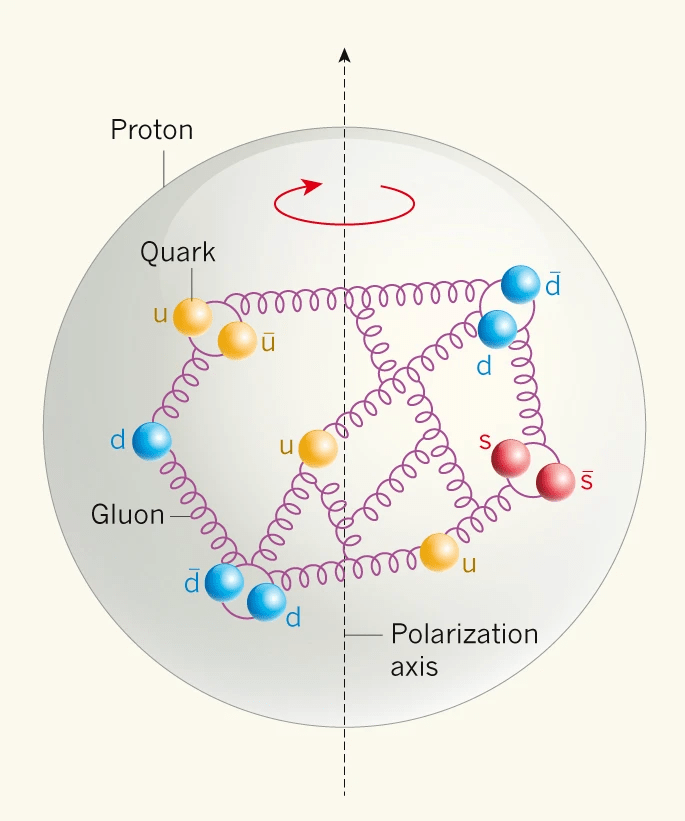
\includegraphics[width=0.35\textwidth]{C:/Users/Carmen/Desktop/Universidad/TFG/Borradores/img/proton.PNG}
	\caption[Estructura interna del protón]
	{Estructura interna de quarks del protón \cite{protonYoung}.}
	\label{fig:proton}
\end{figure}

En la figura \ref{fig:proton}, al margen de los tres quarks de valencia, también se aprecia como el mar de quarks cambia continuamente, al crearse y destruirse parejas $\Pq\Paq$. En concreto, se observa una pareja $\Pqu\Paqu$, dos $\Pqd\Paqd$ y una $\Pqs\Paqs$, pero ya se ha comentado que el protón puede presentar también otras parejas de sabores con menor relevancia para sus propiedades. 

Como se mencionó anteriormente, el estudio de efectos de extrañeza en el protón se ha llevado a cabo en el experimento $Q_{weak}$, cuyo objetivo básico es la determinación de la interacción débil entre el protón y el electrón y, consecuentemente, la medición precisa de la carga débil del protón. Adicionalmente, los estudios de extrañeza y otros sabores ocultos en el protón pueden tener implicaciones profundas en la búsqueda de la materia oscura en el Universo \cite{protonYoung}. 
